

%% NOVAC
%% =============
%%

		\begin{figure}[h]
			\centering
			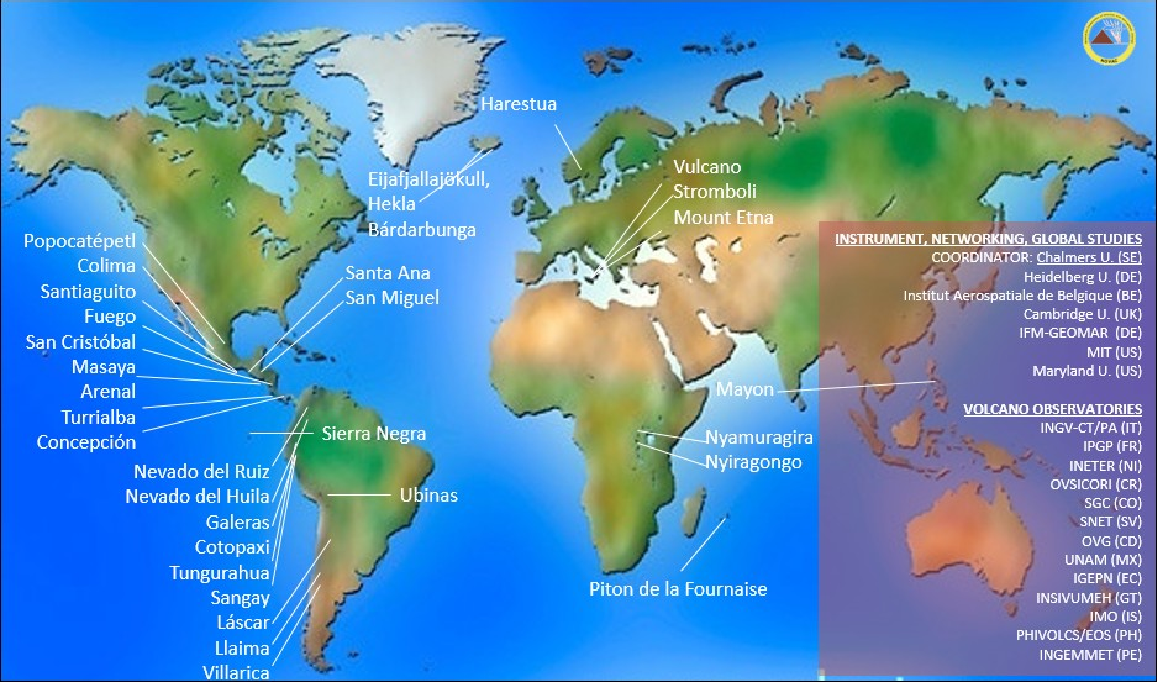
\includegraphics[width=0.8\linewidth]{Bilder/NOVAC2015}
			\caption{Global map of the volcanoes monitored by NOVAC. Used with friendly permission of Santiago Arellano.}
			\label{fig:novac2015}
		\end{figure}
		The Network for Observation of Volcanic and Atmospheric Change (NOVAC) is a network of instruments monitoring volcanoes over the whole world. 
		%
		NOVAC was installed to to add a monitoring parameter for volcanic activity by installing automatised instruments measuring SO2 emissions during daytime.\\
		%
		NOVAC was originally an European funded Research Project from 2005 until 2010. The aim of NOVAC is to  establish  a  global  
		network  of  stations  for  the  quantitative  measurement  of  volcanic gas  emissions in particular SO2. At the beginning, NOVAC encompassed observatories of 15 volcanoes in Africa, America and Europe, including some of the most active and strongest degassing volcanoes in the world. Although the EU-funding has stopped, the network has been constantly growing since it was founded. In 2018 more than 80 instruments are installed at over 30 volcanoes in more than 13 countries.
		\Cref{fig:novac2015} shows a map, with all volcanoes of the Network for Observation of Volcanic and Atmospheric Change.\\
		
		The great advantage of the data monitored in NOVAC is the fact that NOVAC provides continues gas emission data over many years. This ensures statistically meaningful results for the data evaluation.\\
		The instruments used in NOVAC are scanning UV-spectrometer named Mini Doas instruments. \\
		The  Mini DOAS  instrument  represents  a  major  breakthrough  in  volcanic  gas	monitoring as it is capable of real-time semi-continuous unattended measurement of the total emission fluxes of  \ce{SO2} and BrO from a volcano. Semi-continues in this case means that the measurement is only possible during daytime.\\
		%
		\begin{figure}
			\centering
		%	\subfigure[ ]
		 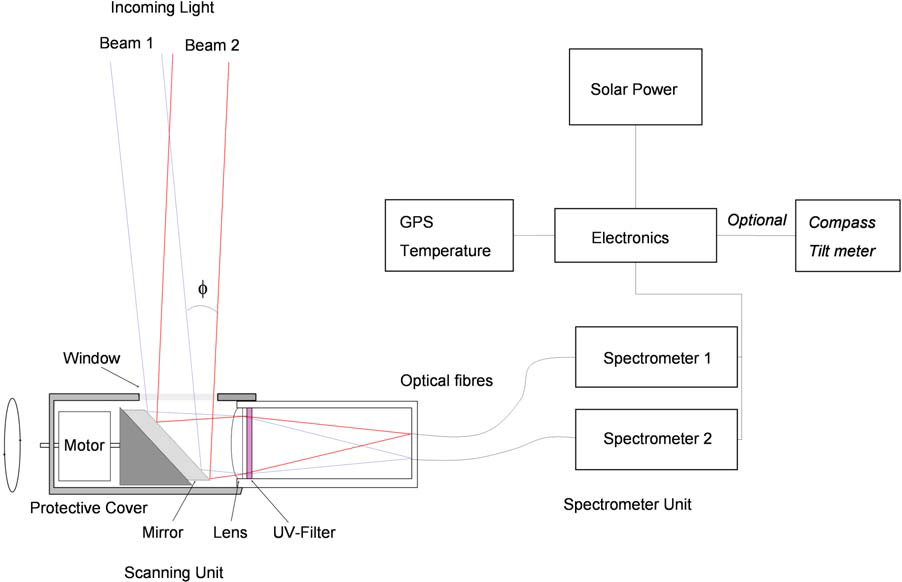
\includegraphics[width=1\textwidth]{Bilder/Simon/Bilder_Tung/NOVAC_Instrument}
		%	\subfigure[Different Scan geometrys of NOVAC-Instruments From \cite{galle2010network}]{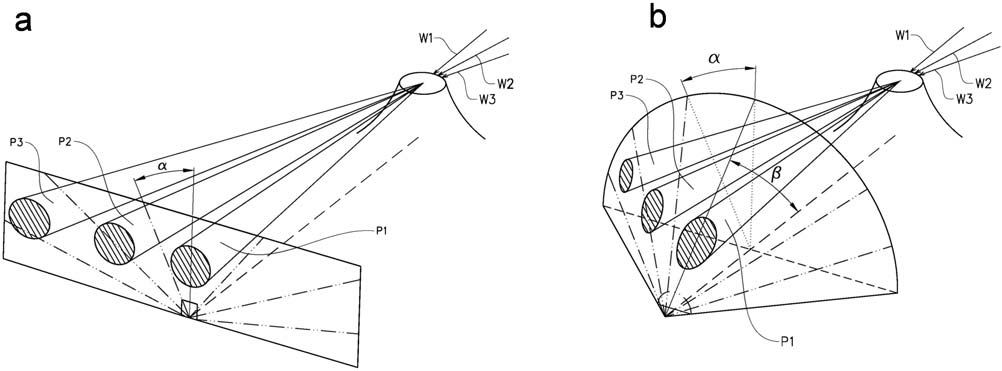
\includegraphics[width=0.49\textwidth]{Bilder/Simon/Bilder_Tung/NOVAC_scan_geo}}
			\caption{schematic sketch of a NOVAC instrument. From \cite{galle2010network}}
		\end{figure}
		The  basic  Mini DOAS  system  consists  of  a  pointing  telescope  fiber-coupled  to  a  spectrograph.  
		Ultraviolet light from the sun, scattered from aerosols and molecules in the atmosphere, is collected by 
		means  of  a  telescope  with  a  quartz  lens  defining  a  field-of-view  of  12~mrad
		\citep{NOVACsite}. \\
		The spectrometers measure in the UV region in a wavelength range of 280 to 420~nm. In this range the differential structures of \ce{SO2} and BrO structures are dominant.\\
		The lack of temperature stabilization at the instruments used by NOVAC comes with a reduced precision of the data, but the huge amount of data produced by NOVAC compensates for this limitation.  
%		\textcolor{red}{naja und es kommt evben auch immer drauf an was fuer genauigkeiten man bracuht - wenn ich eine groessenordnung in der emissionsmessungen sehen will muss ich nicht auf ein promille genau messen,..}
		
		\section{Measurement routine}
		\begin{figure}[h]
			\centering
			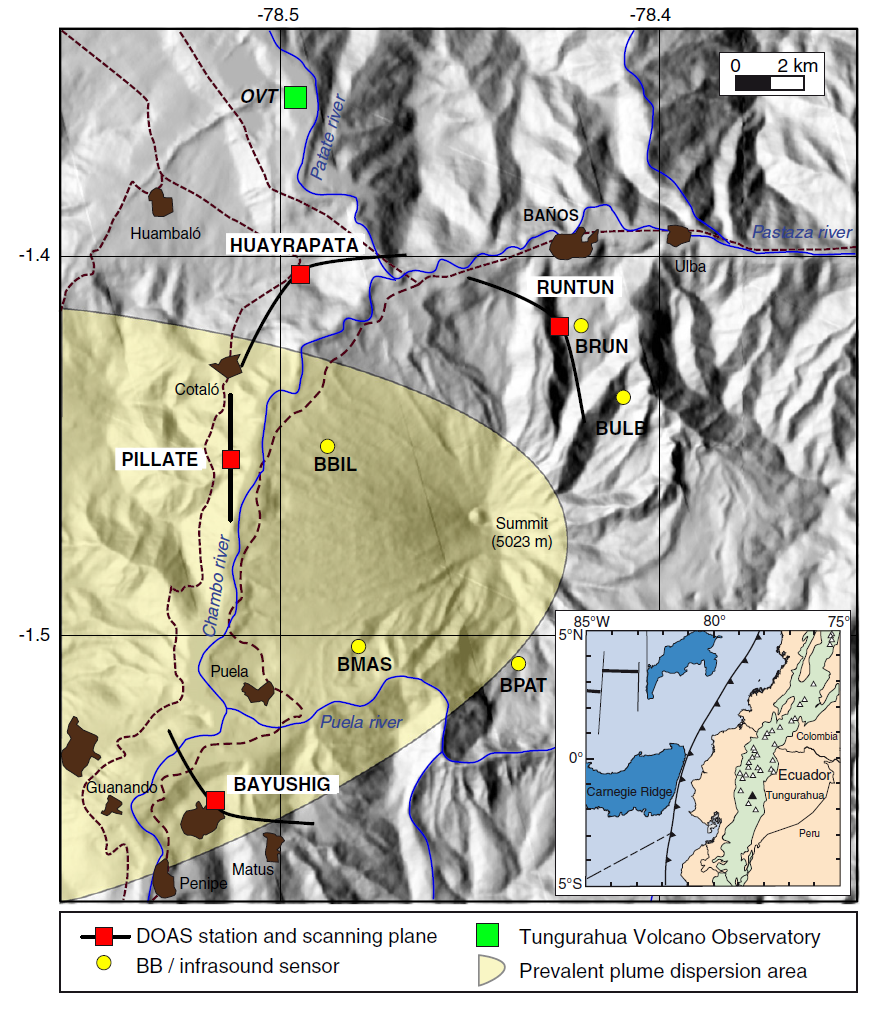
\includegraphics[width=0.6\linewidth]{Bilder/Simon/Bilder_Tung/Map_Tungurahua2}
			\caption{Topographig Map of the Tungurahua Volcano. The predominant plume direction is shaded in yellow.  Four NOVAC stations are shown as red squares, the corresponding scanning geometry is sketched with black lines. From \cite{hidalgo2015so2}.}
			\label{fig:maptungurahua2}
		\end{figure}
		The instruments are set up five to ten km downwind of the volcano. To cover most of the occurring wind directions two to five instruments are installed at each volcano. Ideally, the measurement plane is orthogonal to the plume, to get the best measurement results. In reality, the measurement plane might be rotated.\\
		
		For the calculations of gas data from the DOAS retrieval a scan of the Plume and a scan without any volcanic trace gases (reference spectrum) is needed.  The is done without any knowledge of the plume location by scanning the whole sky. 
		The measurement routine starts with a spectrum in zenith direction: the pre-reference. The exposure time of the pre-reference will be used for the whole scan.
		Afterwards, the dark current spectrum is recorded for the correction of the dark and offset\\
		Then the instrument turns automatically to the side, recording spectra at the elevation angle from -90$^{\circ}$ to 90$^{\circ}$ with steps of 3.6$^{\circ}$. \\
		The instruments records 53 spectra per scan, the pre-reference, the dark current spectrum and 51 spectra at different elevation angles.
		One whole measurement cycle from horizon to horizon ans takes 6 to 15 minutes.